% Chapter Template

\chapter{The ATLAS Experiment at LHC} % Main chapter title

\label{Chapter3} % Change X to a consecutive number; for referencing this chapter elsewhere, use \ref{ChapterX}

The experimental data for the measurement has been collected by ATLAS detector, one of the detectors placed on LHC at CERN near Geneva city on France-Swiss border. CERN is the largest and most complex high energy physics facility in the world where physicists and engineers from all around the world work together to study the fundamental particles. Since foundation in 1954, many important discoveries have been made at the CERN laboratory. In this chapter, LHC and the ATLAS detector structure are briefly described.%----------------------------------------------------------------------------------------
%	SECTION 1
%----------------------------------------------------------------------------------------

\section{The Large Hadron Collider}
\label{section:LHC}

The LHC is a circular beam collider with a circumference of about 27km designed to accelerate the proton beams with up to a center-of-mass energy of 14 TeV. The collider is situated underground and the deepest point of LHC is 175 meters under the surface. The superconducting magnets cover the whole tunnel to bend the beam, and the project was completed in 2000. There are four main interaction points where the beams collide and the detectors, ALICE, ATLAS, CMS, and LHCb, have been installed to collect the collision data. The acceleration process at CERN involves the chain of accelerators in which each accelerator injects the beam into the next one to bring the beam to higher energies. At last, the beam gets injected to LHC for the final acceleration and collision process.

The beam acceleration started by ionization of hydrogen atoms and separating the protons through an electric field. The protons beam then gets injected to the Linac2, where the protons accelerated up to the 50 MeV. From there, the beam enters the Proton Synchrotron Booster (PSB) and get the energy up to 1.4 GeV. In the next step, the beam gets into the Proton Synchrotron (PS), where the energy of the beam increases to 25 GeV. Afterward, The Super Proton Synchrotron (SPS) accelerates the beam to 450 GeV, which is the last pre-acceleration step before the beam gets injected to LHC. In the LHC, the protons beam divided into two pipes in which one beam accelerated in clockwise and the second beam in the anti-clockwise direction up to 7 TeV. As a result, in the head-to-head collision, the center of mass energy reaches up to 14 TeV, schematic view of acceleration chain is shown in figure \ref{fig:cern}.

\begin{figure}[H]
\centering
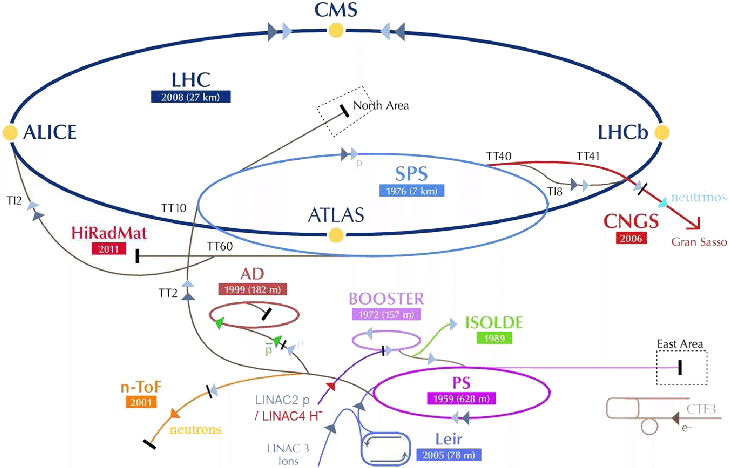
\includegraphics[scale=0.5]{Figures/Schematic-view-of-the-CERN-accelerator-complex.png}
\decoRule
\caption{Schematic view of the CERN accelerators chain, the largest ring in dark blue color is the LHC \cite{cernschematic}.}
\label{fig:cern}
\end{figure}

%----------------------------------------------------------------------------------------
%	SECTION 2
%----------------------------------------------------------------------------------------

\section{ATLAS Detector}
\label{section:ATLAS}

The ATLAS detector is a cylindrical shaped detector with a length of 46m, a diameter of 25m, and it weighs about 7000 tonnes. ATLAS is a multi-purpose detector that is designed to measure the energy and momentum of the particles around the collision point. It uses an orthogonal right-handed coordinate system in which the origin is the center of the detector (interaction point), and the beamline direction defines the $z$-axis, $x$-axis points towards the center of LHC. The $x-y$ plane is perpendicular to the beamline and referred to as the transverse plane. The positive $x$-axis points towards the center of LHC, and the positive $y$-axis points upward to the surface of the earth. The azimuthal angle ($\phi$) is the angle in the transverse plane measured from the $x$-axis, and the polar angle ($\theta$) is the angle in the $y-z$ plane which is often expressed in terms of pseudo-rapidity ($\eta$) and formulated as follows:

\begin{equation}
\eta = - \ln \tan{\frac{\theta}{2}}.
\label{eqn:pseudorapidity}
\end{equation}

The distance between two physical objects defined in terms of pseudo-rapidity and azimuthal angle (which is Lorentz invariant under the boost) as follows:

\begin{equation}
\Delta R = \sqrt{{\Delta\eta}^2 +{\Delta\phi}^2}.
\label{eqn:deltaR}
\end{equation}

The energy and momentum of the particles are expressed in terms of transverse momentum ($p_{T}$) and transverse energy ($E_{T}$); in this way, they are also Lorentz invariant under the boost, defined as follows:

\begin{equation}
p_{T} = \sqrt{{p_{x}}^2 +{p_{y}}^2} = |p|\sin{\theta}, \; E_{T} = |E|\sin{\theta}.
\label{eqn:energymomentum}
\end{equation}

The ATLAS detector provides full coverage of the space around the collision point. The inner structure significant parts can be split into four major components: Inner detector, Calorimeters, Muon Spectrometer, and Magnet system. The Inner detector part (closest part to the collision point) is responsible for detecting the track of charged particles and the position primary and secondary vertices. The calorimeters consist of two inner components, the Electromagnetic Calorimeter (ECAL) and the Hadronic Calorimeter. Energy deposits of the electrons, photons, muons and hadrons are recorded by the calorimeters. The muon spectrometry is the outermost layer of the ATLAS detector. The magnet system can be divided into two parts. The first part is a solenoid magnet that surrounds the inner detector and provides a homogenous magnetic field of 2T to detect the charge and momentum of the particle. The second part consists of three toroidal magnets for barrel and end-caps segments, which provide the trajectory of the muons. A simulated model of the ATLAS detector and the inner structure is given in figure \ref{fig:atlas}. A cross section of the ATLAS detector and the different points at which particles interact with the detector is shown in figure \ref{fig:atlas-cut}.

\begin{figure}[H]
\centering
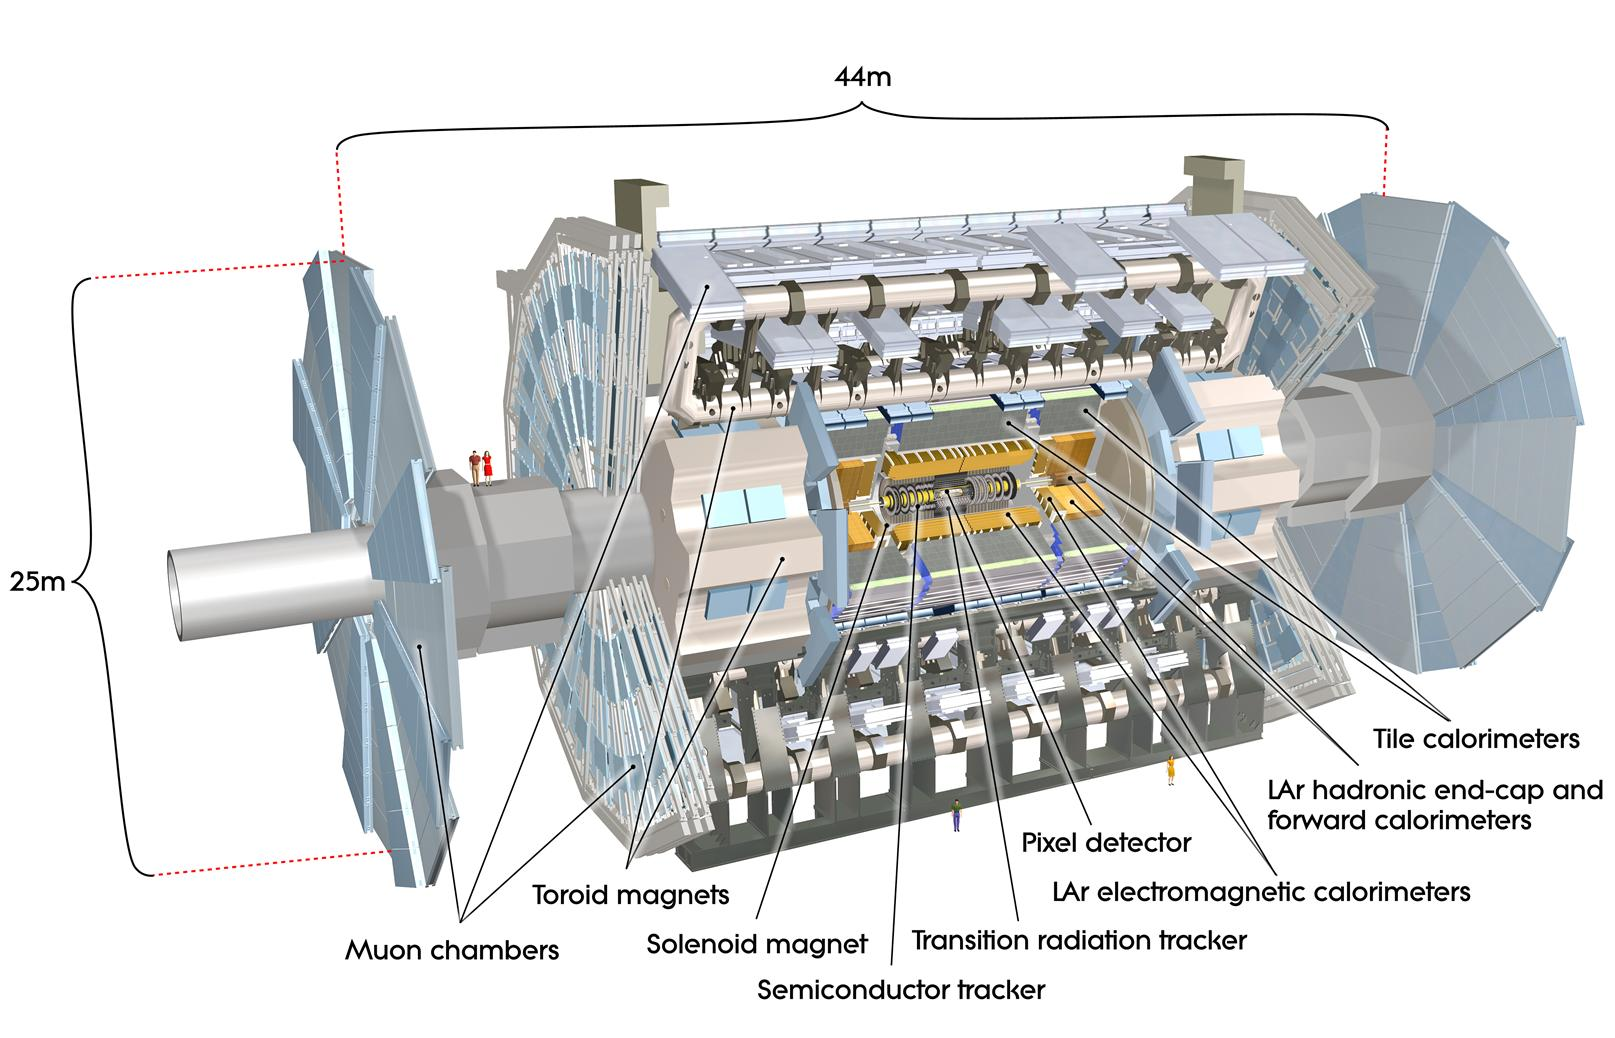
\includegraphics[width=14cm]{Figures/atlas-detector.jpg}
\decoRule
\caption{Schematic view of the ATLAS detector \cite{Pequenao:1095924}.}
\label{fig:atlas}
\end{figure}

\begin{figure}[H]
\centering
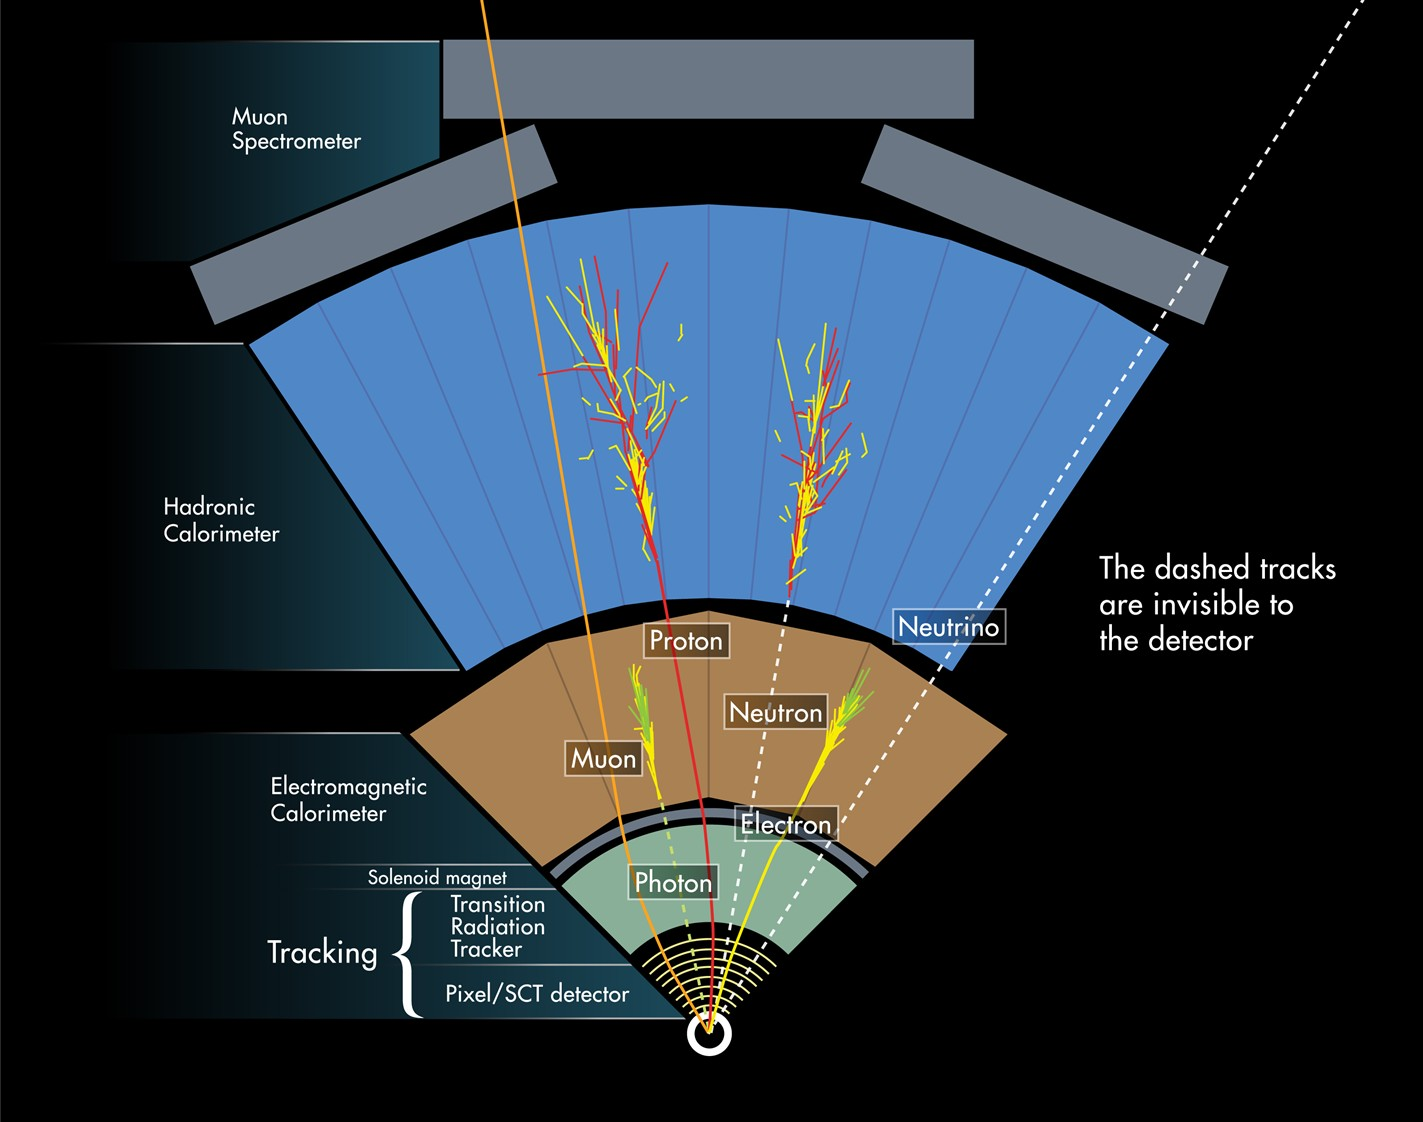
\includegraphics[scale=0.5]{Figures/atlas-cut.jpg}
\decoRule
\caption{A computer simulation overview of the interactions of different particles with the ATLAS subdetectors \cite{Pequenao:1505342}.}
\label{fig:atlas-cut}
\end{figure}

%\section{Event Reconstruction}
%\label{section:reconstruction}
%
%Essential to any successful analysis is the reconstruction, and identification of the physics objects within the ATLAS detector. A combination of the detector's geometry and material composition, as well as advanced algorithms allow physicists to determine the object type, be it a photon, electron, muon, jet, or missing transverse energy. The particles produced in a collision at LHC, pass through the layers of the ATLAS detector and leave a signal on the detector, depending on the type particle. The process of these signals and retrieving the information about the particle and identify it as a physical object, known as reconstruction. The reconstruction of the physical objects starts from the innermost layers of the detector. First, the track and vertices, then the hits on calorimeters and the outer layers information get processed. Then the information from the different layers processed together to reconstruct the physical objects such as electrons and photons.
%Electrons in the ATLAS detector are reconstructed from the energy deposits in ECAL, which are matched to the reconstructed track.
%The reconstruction of photons is carried out in parallel with that of electrons since both objects leave very similar signatures behind in the calorimeter. Nevertheless, being a charged particle, the definition of an electron object is rather straightforward, where the things are a bit more complicated for photons due to their conversion. For this reason, photons are classified into two categories: unconverted and converted photons. Unconverted photons are not associated with any track, and they are simply ECAL clusters. Converted photons are characterized with at least one track originated from a vertex in the ID and associated with a cluster in the ECAL. Therefore, there is a significant similarity between electrons and converted photons.
%
%\begin{figure}[H]
%	\centering
%	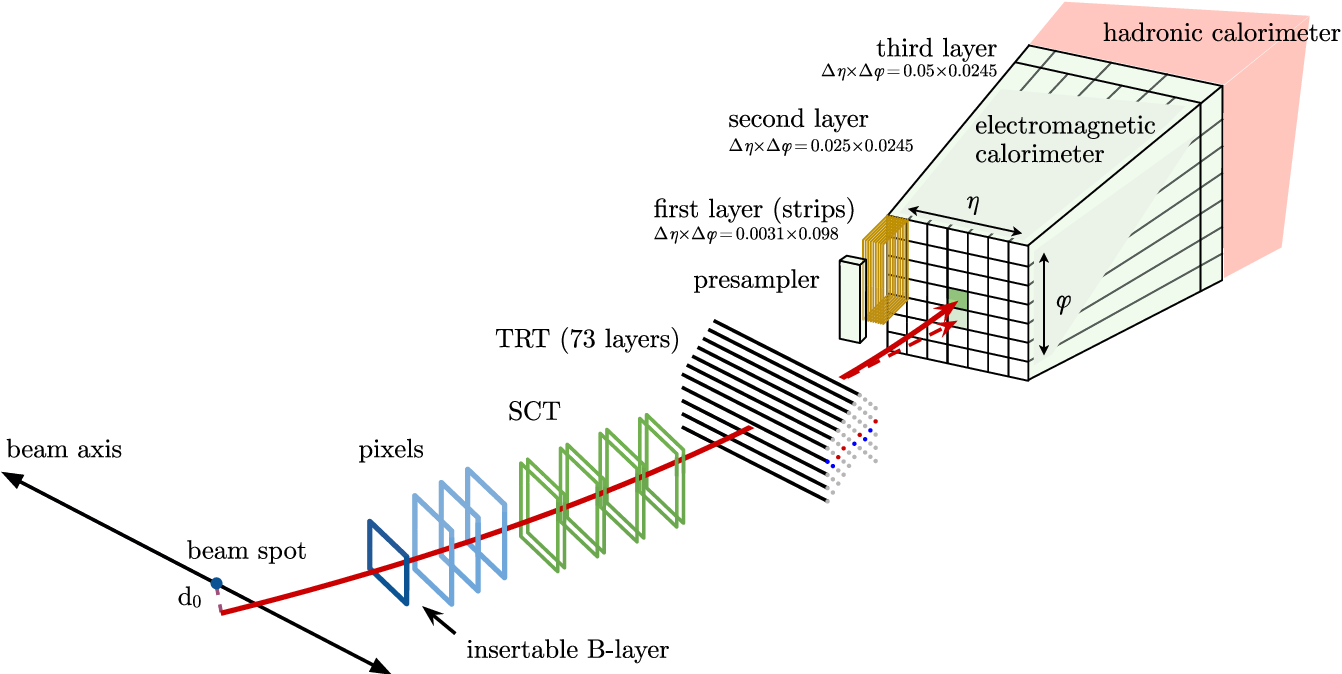
\includegraphics[width=14cm]{Figures/7-Figure1-1.png}
%	\decoRule
%	\caption{A schematic illustration of the path of an electron through the detector. The red trajectory shows the hypothetical path of an electron, which first traverses the tracking system (pixel detectors, then silicon-strip detectors and lastly the TRT) and then enters the electromagnetic calorimeter. The dashed red trajectory indicates the path of a photon produced by the interaction of the electron with the material in the tracking system \cite{s10052-019-7140-6}.}
%	\label{fig:electron-reco}
%\end{figure}
